\scanpage{75}
% archive sheet number: 74
\figure{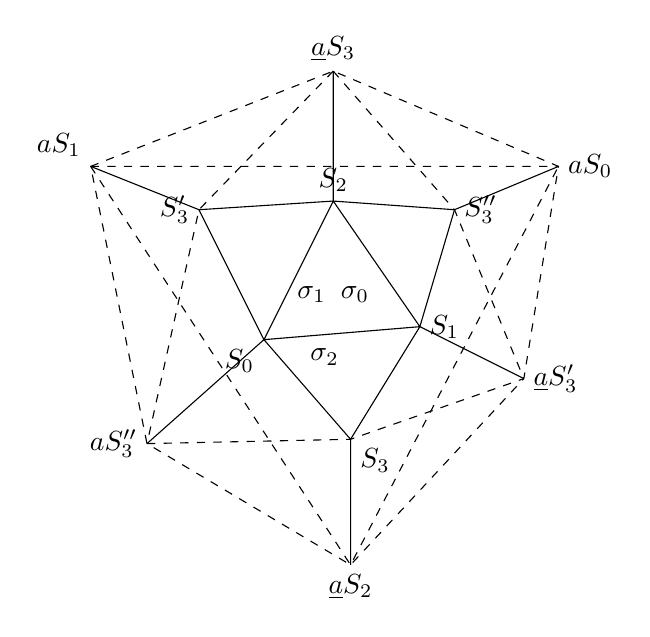
\begin{tikzpicture}[scale=1.1]
\coordinate (s0) at (0,0);\coordinate (s1) at (1.8,.15);\coordinate (s2) at (.8,1.6);\coordinate (s3) at (1,-1.15);
\coordinate (sp) at (-.75,1.5);\coordinate (spp) at (2.2,1.5);
\coordinate (as1) at (-2,2);\coordinate (as0) at (3.4,2);\coordinate (as2) at (1,-2.6);\coordinate (as3) at (.8,3.1);\coordinate (asp) at (3,-.45);\coordinate (aspp) at (-1.35,-1.2);
\draw (s0)--(s1)--(s2)--cycle (s0)--(s3)--(s1) (s0)--(sp)--(s2)--(spp)--(s1);
\draw[dashed] (as1)--(as3)--(as0)--(asp)--(as2)--(aspp)--cycle (as3)--(sp)--(aspp) (as3)--(spp)--(asp) (aspp)--(s3)--(asp);
\draw[dashed,thin] (as1)--(as0) (as1)--(as2)--(as0);
\draw (as1)--(sp) (as0)--(spp) (as3)--(s2) (as2)--(s3) (aspp)--(s0) (asp)--(s1);
\node[below left] at (s0) {$S_0$};\node[right] at (s1) {$S_1$};\node[above] at (s2) {$S_2$};\node[below right] at (s3) {$S_3$};\node[left] at (sp) {$S'_3$};\node[right] at (spp) {$S''_3$};
\node[above left] at (as1) {$aS_1$};\node[right] at (as0) {$aS_0$};\node[below] at (as2) {$\underline aS_2$};\node[above] at (as3) {$\underline aS_3$};\node[right] at (asp) {$\underline aS'_3$};\node[left] at (aspp) {$aS''_3$};
\node at (.55,.52) {$\sigma_1$};\node at (1.05,.52) {$\sigma_0$};\node at (.7,-.2) {$\sigma_2$};
\end{tikzpicture}}
\[
\sigma_0:\quad\begin{aligned}
\inserted{S_0\longrightarrow S_1}\\
\unsure{S_1|S_0}\longleftrightarrow S_0\\
S_2\longmapsto S_2\\S_3\longmapsto S_3
\end{aligned}
\qquad\begin{aligned}
e_1&\longmapsto-e_1\\e_2&\longmapsto-e_1+e_2\\e_3&\longmapsto-e_1+e_3
\end{aligned}
\]
\[
\sigma_0=\begin{pmatrix}-1&-1&-1&1\\0&+1&0&0\\0&0&+1&0\\0&0&0&1\end{pmatrix}
\]
\[
\boxed{\sigma_0(x,y,z)=\deleted{\unsure{\mathrm{id}}}(1-(x+y+z),y,z)}
\]
\figure{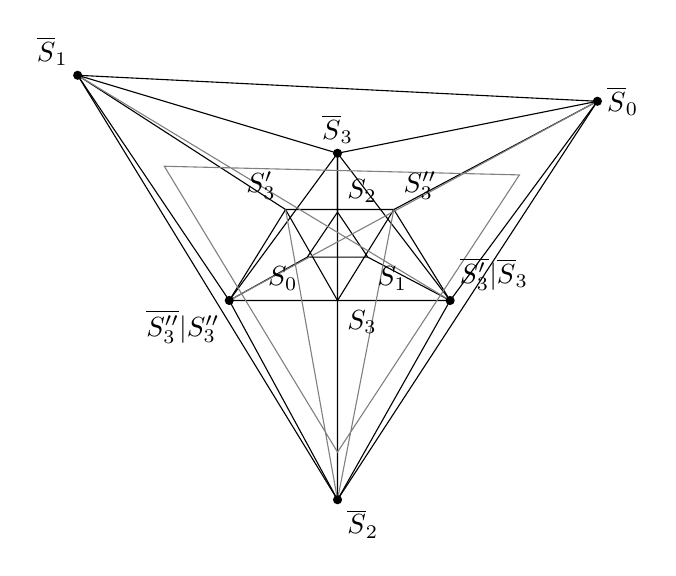
\begin{tikzpicture}[scale=1.1]
\coordinate (A) at (-3,2.6);\coordinate (B) at (3,2.3);\coordinate (C) at (0,-2.3);
\coordinate (t) at (0,1.7);\coordinate (l) at (-1.25,0);\coordinate (r) at (1.3,0);
\coordinate (p) at (-.6,1.05);\coordinate (q) at (.65,1.05);\coordinate (s0) at (-.35,.5);\coordinate (s1) at (.35,.5);\coordinate (s2) at (0,1.02);\coordinate (s3) at (0,0);
\draw (A)--(B)--(C)--cycle (t)--(l)--(r)--cycle;
\draw (A)--(t)--(B) (A)--(p)--(l) (A)--(l) (B)--(q)--(r) (B)--(r) (C)--(l) (C)--(r) (C)--(s3)--(t);
\draw (p)--(q)--(s3)--cycle (s0)--(s1)--(s2)--cycle (l)--(s0) (r)--(s1) (t)--(s2);
\draw[gray,thin] (-2,1.55)--(2.1,1.45)--(0,-1.75)--cycle (A)--(r) (B)--(l) (C)--(p) (C)--(q);
\foreach \P in {A,B,C,t,l,r}{\fill (\P) circle (1.5pt);}
\node[above left] at (A) {$\overline S_1$};\node[right] at (B) {$\overline S_0$};\node[below right] at (C) {$\overline S_2$};\node[above] at (t) {$\overline S_3$};
\node[above left] at (p) {$S'_3$};\node[above right] at (q) {$S''_3$};\node[below left] at (l) {$\unsure{\overline{S''_3}|S''_3}$};\node[above right] at (r) {$\unsure{\overline{S'_3}|\overline S_3}$};
\node[below left] at (s0) {$S_0$};\node[below right] at (s1) {$S_1$};\node[above right] at (s2) {$\unsure{S_2}$};\node[below right] at (s3) {$S_3$};
\end{tikzpicture}}
\[
\sigma_1:\quad\begin{aligned}
S_0&\longmapsto S_0\\S_1&\longmapsto S_2\\S_2&\longmapsto S_1\\S_3&\longmapsto S'_3=S_0+(1+\alpha)(e_2-e_1)+e_3
\end{aligned}
\qquad\begin{aligned}
e_1&\longmapsto e_2\\e_2&\longmapsto e_1\\e_3&\longmapsto(1+\alpha)(e_2-e_1)\inserted{+e_3}\\
&=\alpha'e_1-\alpha'e_2+e_3
\end{aligned}
\]
\[
\sigma_1=\begin{pmatrix}0&1&\alpha'&0\\1&0&-\alpha'&0\\0&0&1&0\\0&0&0&1\end{pmatrix}
\qquad\boxed{\sigma_1(x,y,z)=(y+\alpha'z,x-\alpha'z,z)}
\]
\[
\sigma_2:\quad\begin{aligned}
S_0&\longmapsto S_0\\S_1&\longmapsto S_1\\S_2&\longmapsto S_3\\S_3&\longmapsto S_2
\end{aligned}
\qquad\begin{aligned}
e_1&\longmapsto e_1\\e_2&\longmapsto e_3\\e_3&\longmapsto e_2
\end{aligned}
\]
\[
\sigma_2=\begin{pmatrix}1&0&0&0\\0&0&1&0\\0&1&0&0\\0&0&0&1\end{pmatrix}
\quad\deleted{\unsure{=}}\boxed{\sigma_2(x,y,z)=(x,z,y)}
\]
\[
\left\{\begin{aligned}
H_0:&\quad2x+y+z-1=0\\H_1:&\quad x-y-\alpha'z=0\\H_2:&\quad y-z=0
\end{aligned}\right.
\qquad\left\{\begin{aligned}
\Delta_0:&\quad y=z=0&&\text{i.e. }\Delta_0=\unsure{\underline O_S|\mathcal O_S}\cdot e_1\\
\Delta_1:&\quad z=0,x+y=0&&\text{i.e. }\Delta_{\unsure{1|p}}=\underline O_S(e_1-e_2)\\
\Delta_2:&\quad x=0,y+z=0&&\text{i.e. }\Delta_2=\underline O_S(e_2-e_3)
\end{aligned}\right.
\]
en car. $2$, $H_2\parallel H_0$.
\[
\left\{\begin{aligned}
D_0=H_1\cap H_2:&\quad y=z=\alpha'x\\
D_1=H_2\cap H_0:&\quad y=z=\underbrace{\tfrac12-x}_{\text{(car}\ne2\text{)}}\\
D_2=H_0\cap H_1:&\quad y=\deleted{\unsure{\alpha}}(1-3\alpha)x+\alpha,\quad z=\unsure{-3|3}(1-\alpha)x+(1-\alpha)
\end{aligned}\right.
\]
\[
\begin{aligned}
D_0&=\underline O_S(1,\alpha',\alpha')=\underline O_S(-\alpha,1,1)\\
\underline{\mathrm{hom}\,D_1}:\ (y=z=-x)&=\underline O_S(1,-1,-1)\\
\underline{\mathrm{hom}}(D_2)&=\underline O_S(1,1-3\alpha,\unsure{-3|3}(1-\alpha))
\end{aligned}
\]
\uline{centre}\quad $o=\frac12(\alpha',1-\alpha',1-\alpha')=\deleted{\unsure{\frac12\alpha'}}$

\uline{Antipodisme}
\[
\underline a(x,y,z)=(\alpha'-x,(1-\alpha')-y\unsure{\},},(1-\alpha')-z\unsure{\}})
\]
\[
\tfrac12(-1+\sqrt5\quad\unsure{)|?}=-\unsure{?|2|1}+\unsure{\sqrt5|\sqrt\gamma}
\]
